\documentclass{beamer}

\usepackage{graphicx}
\graphicspath{ {./images/} }
\usepackage[utf8]{inputenc}
\usepackage{hyperref}


%Information to be included in the title page:
\title{1.3 Weierstraß Normalform\\1.4 Explizit Formulas for the Group Law}
\author{Luca Leon Happel}

\date{31 Mai 2021}



\begin{document}
\setbeamertemplate{navigation symbols}{}

\frame{\titlepage}

\begin{frame}
\frametitle{Erinnerung}
	\textbf{Mordell's Theorem}\\
	Wenn eine nicht singuläre rationale kubische Kurve in der
	Ebene einen rationalen Punkt hat, so ist die Gruppe der
	rationalen Punkte endlich erzeugt.\\
	Möchten wir beweisen!
\end{frame}

\begin{frame}
\frametitle{vereinfachen}
	Um dies beweisen zu können, müssen wir unsere
	Ausgangssituation vereinfachen!
\end{frame}

\begin{frame}
\frametitle{Kubische Kurve}
    \begin{figure}
		\caption{$C:ax^3+bx^2y+cxy^2+dy^3+ex^2+fxy+gy^2+hx+iy+j=0$}
		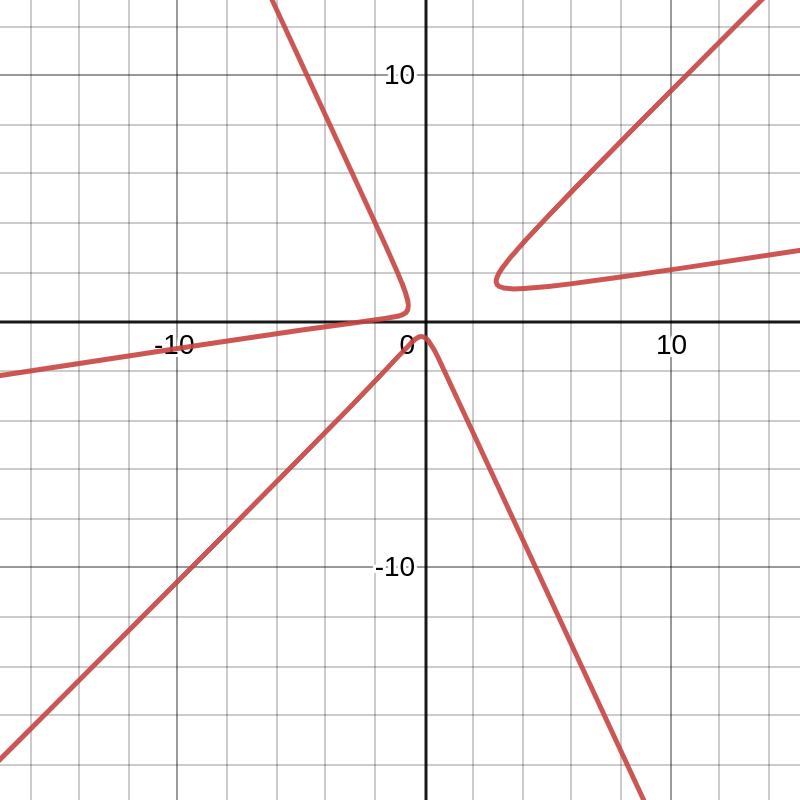
\includegraphics[scale=0.3]{images/desmos-graph01.png}
    \end{figure}
\end{frame}

\begin{frame}
\frametitle{allgemeine Weierstraß Normalform}
    \begin{figure}
		\caption{$C: P=0 \to C': y^2=x^3+ax^2+bx+c$}
		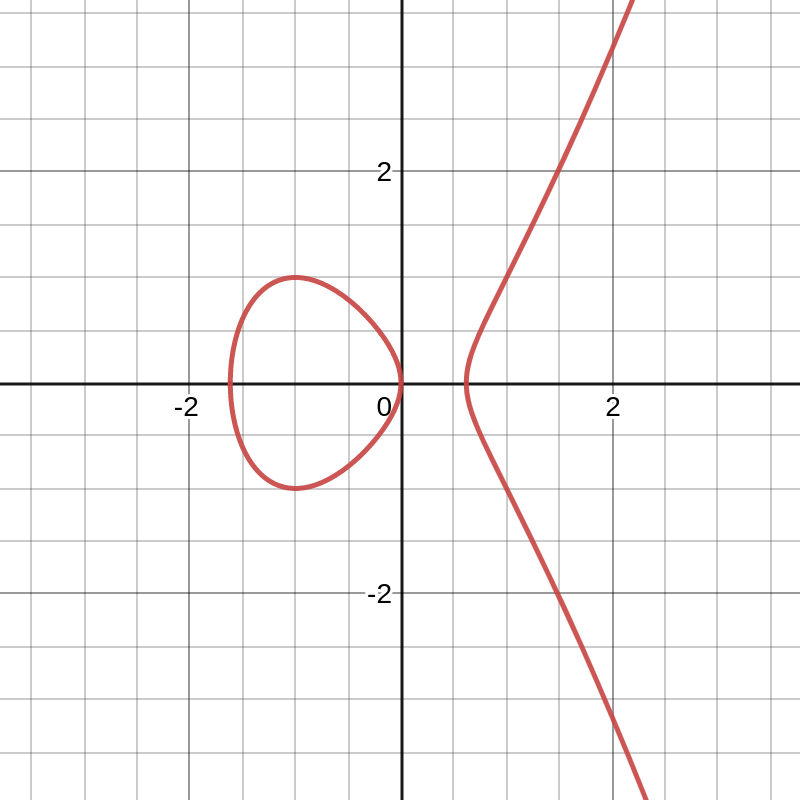
\includegraphics[scale=0.3]{images/desmos-graph02.png}
    \end{figure}
\end{frame}

\begin{frame}
\frametitle{Weierstraß Normalform}
	Es gibt die klassische Weierstraß Normalform
	\[y^2=4x^3-g_2x-g_3\]
	und die allgemeine Weierstraß Normalform
	\[y^2=x^3+ax^2+bx+c\]
	wobei die Koeffizienten jeweils rational sind. Wir werden die
	allgemeine betrachten. Die WNF erlaubt uns, einfacher mit
	elliptischen Kurven umzugehen, da jede elliptische Kurve
	birational äquivalent zu einer WNF ist.
\end{frame}

\begin{frame}
\frametitle{Konstruktion der Weierstraß Normalform - Schritt 1}
	Sei \(C\) eine kubische Kurve im Projektiven Raum
	mit \(\mathcal{O}\), einem rationalen Punkt auf \(C\).
	Verändere/wähle Achsen so, dass wir eine einfachere Form
	erhalten.
\end{frame}

\begin{frame}
\frametitle{Konstruktion der Weierstraß Normalform - Schritt 1}
    \begin{center}
    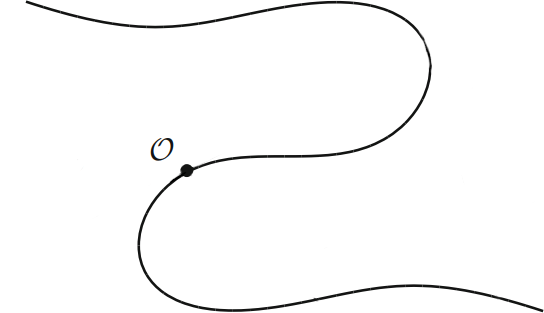
\includegraphics[scale=2]{images/WNF_Konstruktion_1.png}
    \end{center}
\end{frame}

\begin{frame}
\frametitle{Konstruktion der Weierstraß Normalform - Schritt 2}
	Wir nehmen die Tangente von \(\mathcal{O}\) und verwenden
	sie als unser \(Z=0\), also unsere \(Z\)-Achse.
\end{frame}

\begin{frame}
\frametitle{Konstruktion der Weierstraß Normalform - Schritt 2}
    \begin{center}
    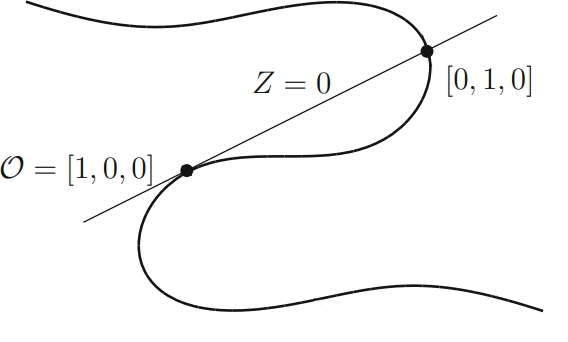
\includegraphics[scale=2]{images/WNF_Konstruktion_2.png}
    \end{center}
\end{frame}

\begin{frame}
\frametitle{Konstruktion der Weierstraß Normalform - Schritt 3}
	Diese Tangente schneidet die Kurve an einer weiteren Stelle
	\((0:1:0)\) und die Tangente an dieser Stelle wird unsere
	\(X\)-Achse.
	\\
	Wenn \(\mathcal{O}\) ein Wendepunkt (point of inflection) ist,
	können wir eine beliebige Gerade wählen, welche nicht durch
	\(\mathcal{O}\) geht.
\end{frame}

\begin{frame}
\frametitle{Konstruktion der Weierstraß Normalform - Schritt 3}
    \begin{center}
    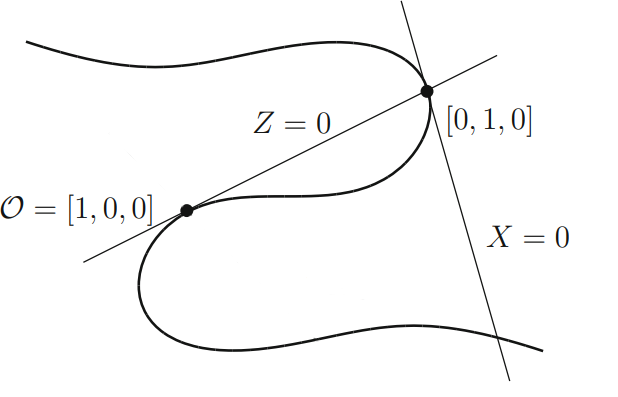
\includegraphics[scale=2]{images/WNF_Konstruktion_3.png}
    \end{center}
\end{frame}

\begin{frame}
\frametitle{Konstruktion der Weierstraß Normalform - Schritt 4}
	Zuletzt wählen wir noch eine beliebige Gerade, welche durch
	\(\mathcal{O}\) geht als unsere \(Y\)-Achse
\end{frame}

\begin{frame}
\frametitle{Konstruktion der Weierstraß Normalform - Schritt 4}
    \begin{center}
    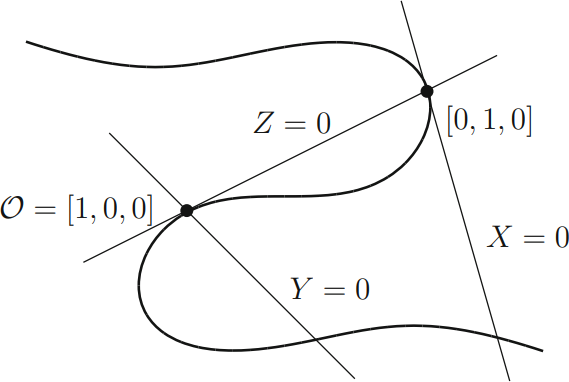
\includegraphics[scale=2]{images/WNF_Konstruktion_4.png}
    \end{center}
\end{frame}

\begin{frame}
\frametitle{Konstruktion der Weierstraß Normalform - Schritt 5}
	\[\underbrace{x=\frac{X}{Z}, \quad y=\frac{Y}{Z}}_{\text{Projektive Transformation}}\]
	Neue Form der Gleichung:
	\[xy^2+(ax+b)y=cx^2+dx+e\]
	Auf beiden Seiten mit \(x\) multiplizieren:
	\[(xy)^2+(ax+b)xy=cx^3+dx^2+ex\]
\end{frame}

\begin{frame}
\frametitle{Konstruktion der Weierstraß Normalform - Schritt 6}
	Benenne \(xy\) in \(y\) um:
	\[y^2+(ax+b)y=cx^3+dx^2+ex\]
	Benenne \(\left(y-\frac{ax+b}{2}\right)\) in \(y\)
	(lineare Transformation) um, was effektiv durch quadratische
	Ergänzung unser Resultat:
	\[y^2 = \text{kubische Funktion in } x\]
\end{frame}

\begin{frame}
\frametitle{Beispiel}
	Betrachten wir das Beispiel $u^3+v^3=\alpha$ für
	$\alpha \in\mathbb{Q}$
\end{frame}

\begin{frame}
\frametitle{Beispiel}
    \begin{center}
    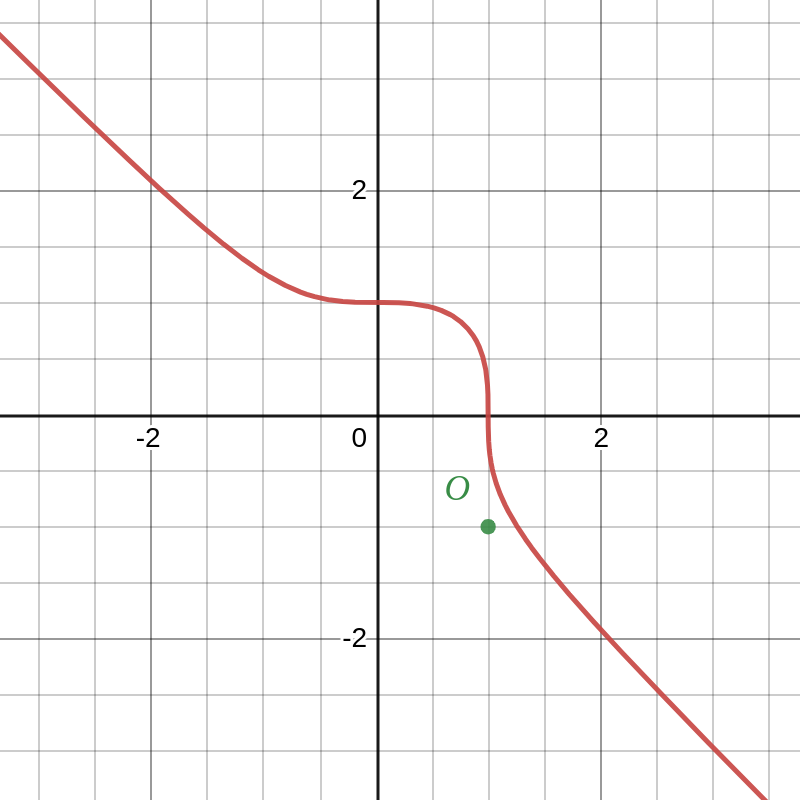
\includegraphics[scale=0.3]{images/desmos-graph03.png}
    \end{center}
\end{frame}

\begin{frame}
\frametitle{Beispiel - Schritt 1}
	Zuerst projektivieren wir und erhalten $U^3+V^3 = \alpha W^3$.
	Wir können leicht sehen, dass \(\mathcal{O}=(1:-1:0)\) eine Lösung
	ist. Weil \(\mathcal{O}\) ein inflection point ist, können wir
	\(X=0\) fast frei wählen (wir dürfen die $X$-Achse nur nicht gleich
	der $Y$- oder der $Z$- Achse wählen).
	Schlussendlich erhalten wir
	\[x=\frac{12\alpha}{u+v}, \quad y=36\alpha\frac{u-v}{u+v}\]
\end{frame}

\begin{frame}
\frametitle{Beispiel - Schritt 2}
	Durch Umformungen erkennen wir, dass \(x,y\) die Weierstraß
	Normalform $y^2=x^3-432\alpha^2$ erfüllen.
	Explizit können wir dies nachprüfen, indem wir \(u,v\) einsetzen
	und ausmultiplizieren. So erhalten wir
	\[
		- \frac{1728 \alpha^{3}}{\left(u + v\right)^{3}} + \frac{1296 \alpha^{2} \left(u - v\right)^{2}}{\left(u + v\right)^{2}} + 432 \alpha^{2}
	\]
\end{frame}

\begin{frame}
\frametitle{Beispiel - Schritt 3}
	Ausmultiplizieren ergibt:
	\[ - \frac{1728 \alpha^{3}}{u^{3} + 3 u^{2} v + 3 u v^{2} + v^{3}} + \frac{1296 \alpha^{2} u^{2}}{u^{2} + 2 u v + v^{2}} \]
	\[- \frac{2592 \alpha^{2} u v}{u^{2} + 2 u v + v^{2}} + \frac{1296 \alpha^{2} v^{2}}{u^{2} + 2 u v + v^{2}} + 432 \alpha^{2}\]
	Wir können dies nun vereinfachen:
	\[ \frac{1728 \alpha^{2} \left(- \alpha + u^{3} + v^{3}\right)}{u^{3} + 3 u^{2} v + 3 u v^{2} + v^{3}} \]
	Wir sehen also, dass wenn \(y^2=x^3-432\alpha^2\) eine Lösung
	hat, so hat auch \(u^3+v^3=\alpha\) eine Lösung.
\end{frame}

\begin{frame}
\frametitle{Beispiel - Schritt 4}
	Wir können den Prozess auch rückwärts gehen und \(u,v\) durch
	\(x,y\) darstellen, indem wir
	$u=\frac{36\alpha+y}{6x}$ und $v=\frac{36\alpha-y}{6x}$ verwenden.
	\\
	Wenn wir rationale Lösungen für \(y^2=x^3-432\alpha^2\) haben,
	so haben wir auch rationale Lösungen für \(u^3+v^3=\alpha\) und
	umgekehrt auch.
	\\
	Es gibt nur endlich viele Ausnahmen (z.B. wenn \(u=-v\))
	aber diese sind schnell zu finden.
\end{frame}

\begin{frame}{Theorem von Mordell(1922)}
    Sei \(C\) eine nicht-singuläre kubische Kurve, dann gibt es eine endliche Menge von rationalen Punkten, so dass alle anderen rationalen Punkte duch wiederholtes Geraden ziehen und schneiden erhalten werden können.
\end{frame}

\begin{frame}{Existenz}
    Es gibt leider noch keine Methode die in endlich vielen Schritten feststellt, ob eine über \(\mathbb{Q}\) definierte kubische Kurve \(C\subset\mathbb{P}^{2}(\mathbb{C})\) einen rationalen Punkt besitzt. Es gibt kein Analogon von Hasse's Therorem für kubische Kurven.
\end{frame}

\begin{frame}{Annahme}
    Um dieses schwierige Problem zu Umgehen werden wir von nun an annehmen das unsere kubische Kurve \(C\subset\mathbb{P}^{2}(\mathbb{C})\) einen rationalen Punkt hat, den wir \(\mathcal{O}\) nennen.
\end{frame}

\begin{frame}{Verknüpfung II}
   Wenn wir zwei rationale Punkte auf einer über \(\mathbb{Q}\) definierten kubischen Kurve \(C\subset\mathbb{P}^{2}(\mathbb{C})\) haben, sagen wir \(P\) und \(Q\). Dann sieht \(\ast\) aus wie eine Verknüpfung auf der Menger aller rationalen Punkte auf \(C\), die ein Paar \((P,Q)\) zum Punkt \(P\ast Q\) schickt. Was für eine algebraische Struktur liefert uns diese Verknüpfung?
\end{frame}

\begin{frame}{Gruppe}
    Eine Gruppe? Leider nicht, da man leicht sieht, dass es kein neutrales Element gibt.\newline
    Aber durch ausprobieren, können wir die Menge der rationalen Punkte zu einer kommutativen Gruppe machen, wobei das neutrale Element gegeben ist durch \(\mathcal{O}\).
\end{frame}

\begin{frame}{Addition}
Die Addition dieser Gruppe ist gegeben durch
\[P+Q=\mathcal{O}\ast(P\ast Q)=Q+P\]
\begin{center}
% \includegraphics[scale=0.3]{images/3.PNG}
\end{center}
Müssen also nur noch verifizieren, dass die Addition den Gruppenaxiomen genügt.
\end{frame}

\begin{frame}{Neutrales Element}
\[P+\mathcal{O}=P\]
\begin{center}
% \includegraphics[scale=0.3]{images/4.PNG}
\end{center}
\end{frame}

\begin{frame}{Inverse}
\[Q+(-Q)=\mathcal{O}\]
\begin{center}
% \includegraphics[scale=0.3]{images/5.PNG}
\end{center}
\end{frame}

\begin{frame}{Assoziativ}
\[(P+Q)+R=P+(Q+R)\] um dies zu zeigen, reicht es zu zeigen, dass \[(P+Q)\ast R=P\ast(Q+R)\]
\end{frame}

\begin{frame}{Assoziativ}
\begin{center}
% \includegraphics[scale=0.3]{images/6.PNG}
\end{center}
\end{frame}

\begin{frame}{Assoziativ}
    Jeder der Punkte
    \[\mathcal{O},P,Q,R,P\ast Q,P+Q,Q\ast R, Q+R\quad(\ast\ast\ast)\]
    liegt auf einer gestrichelten oder einer der durchgezogenen Geraden. Wenn der Schnittpunkt der gestrichelten Gerade durch \(P+Q\) und \(R\) und der durchgezogenen Gerade durch \(P\) und \(Q+R\) auf der kubischen Kurve liegt, haben wir gezeigt, dass \[(P+Q)\ast R=P\ast(Q+R)\]
\end{frame}

\begin{frame}{Bezout's Theorem}
    Der Schnitt \(X\cap Y\) von zwei allgemeinen Kurven \(X,Y\subset\mathbb{P}^{2}(\mathbb{C})\) von Grad \(m,n\geq1\) besteht aus mn Punkten. In unserem Fall also 9 Punkten
    \begin{center}
        % \includegraphics[scale=0.3]{images/2.PNG}
    \end{center}
\end{frame}

\begin{frame}{Lemma}
    Wir wollen folgendes Lemma benutzen:\newline
    \begin{quote}
    Seien \(C,C_{1}\) und \(C_{2}\) kubische Kurven.Angenommen \(C\) geht durch 8 der 9 Schnittpunkte von \(C_{1}\) und \(C_{2}\). Dann geht \(C\) auch durch den 9. Schnittpunkt.
    \end{quote}
\end{frame}

\begin{frame}{Beweis I}
    Um eine kubische Kurve \(C\) zu definieren brauchen wir 10 Koeffizienten, wobei das multiplizieren dieser Koefizienten mit einer Einheit die gleiche Kurve liefert. Können uns also die Menge aller kubischen Kurve als 9-dimensional vorstellen. Wenn wir jetzt fordern, dass die kubischen Kurven durch einen gegebenen Punkt gehen, stellt dies eine lineare Bedingung an die Koeffizienten des kubischen Polynoms. Die Menge aller kubischen Kurve die durch einen gegebenen Punkt gehen ist also nur noch 8-dimensional. Induktiv erreichen wir, dass die Familie aller kubischen Kurven die durch die 8 Schnittpunkte \(P_{1},\dots,P_{8}\) von \(C_{1}\) und \(C_{2}\) gehen 1-dimensional ist.
\end{frame}

\begin{frame}{Beweis II}
    Seien \(F_{1}(x,y)=0\) und \(F_{2}(x,y)=0\) die kubischen Gleichung von \(C_{1}\) und \(C_{2}\). Dann ist für jede Wahl von \(\lambda_{1}\) und \(\lambda_{2}\), die Linearkombination \(\lambda_{1}F_{1}+\lambda_{2}F_{2}\) ist eine kubische Kurve, die durch \(P_{1},\dots,P_{8}\) geht. Da die Familie solcher kubischen Kurven 1-dimensional ist, muss \(\lambda_{1}F_{1}+\lambda_{2}F_{2}\) diese Familie sein. Insbesondere ist die kubische Kurve \(C\) gegeben durch die Gleichung \(\lambda_{1}F_{1}+\lambda_{2}F_{2}=0\) für geeignetes \(\lambda_{1}\) und \(\lambda_{2}\).
\end{frame}

\begin{frame}{Beweis III}
    Da \(P_{9}\) auf \(C_{1}\) und \(C_{2}\) liegt, verschwinden \(F_{1}(x,y)\) und \(F_{2}(x,y)\) beide in \(P_{9}\). Daraus folgt, dass auch \(\lambda_{1}F_{1}+\lambda_{2}F_{2}\) in \(P_{9}\) verschwindet, also liegt \(P_{9}\) auch in \(C\).
\end{frame}

\begin{frame}{Assoziativ}
    Wir haben 9 Punkte, nämlich die genannten 8 Punkte und den Schnittpunkt der gestrichelten und durchgezogenen Gerade. Wir haben also zwei (degenerierte) kubische Kurven die durch 9 Punkte gehen, da eine Gerade durch eine lineare Gleichung gegeben ist und die Multiplikation von drei linearen Gleichungen eine kubische Gleichung ist. Die Lösungsmenge dieser ist einfach die Vereinigung der drei Geraden.
\end{frame}

\begin{frame}{Assoziativ}
    Sei \(C_{1}\) die Vereinigung der drei gestrichelten Geraden und \(C_{2}\) die Vereinigung der drei durchgezogenen Geraden. Per Konstruktion gehen die zwei kubischen Kurven durch die 9 Punkte. Die originale kubische Kurve \(C\) geht durch die 8 Punkte gegeben in \((\ast\ast\ast)\) und somit nach Lemma auch durch den Neunten. Damit haben wir gezeigt
    \[(P+Q)\ast R=P\ast(Q+R)\]
\end{frame}

\begin{frame}{Mordell's Theorem}
    Haben also folgende Umformulierung von Mordell's Theorem:
    \begin{quote}
        \textbf{Mordell's Theorem}. Wenn eine nicht-singuläre rationale kubische Kurve einen rationalen Punkt hat, dann ist die Gruppe der rationalen Punkte endlich erzeugt.
    \end{quote}
    Diese Version ist natürlich deutlich besser, da wir nun elementare Gruppentheorie benutzen können für den Beweis.
\end{frame}

\begin{frame}{Bemerkungen I}
    Die Wahl von \(\mathcal{O}\) ist bei allen Betrachtungen nicht von Bedeutung. Wenn wir ein anderes \(\mathcal{O}'\) als neutrales Element wählen, dann bekommen wir eine Gruppe mit der selben Struktur. Denn die Abbildung
    \[P\rightarrow P+\mathcal{O}'\]
    ist ein Isomorphismus von der Gruppe \((C,\mathcal{O},+)\) zu der Gruppe \((C,\mathcal{O}',+')\), wobei die neue Addition gegeben ist durch
    \[P+'Q=P+Q-\mathcal{O}'\]
\end{frame}

\begin{frame}{Bemerkungen II}
    Wenn die Gerade durch \(P\) und \(Q\) tangent zur Kurve in \(P\) ist, dann muss der dritte Schnittpunkt, als \(P\) interpretiert werden. Und wenn du die Tangente als Gerade durch \(P\) und \(P\) deutest, ist der dritte Schnittpunkt \(Q\). Wenn \(P\) ein Inflektionspunkt von \(C\)
    ist, dann trifft die Tangente in \(P\) die Kurve dreimal in \(P\). In diesem Fall ist der dritte Schnittpunkt für die Gerade durch \(P\) und \(P\) wieder \(P\). In anderen Worten, wenn \(P\) ein Inflektionspunkt ist, dann \(P\ast P=P\).
\end{frame}
\end{document}
